\item \points{4b}
\textbf{The double descent phenomenon for unregularized models}

In this question, you will empirically observe the double descent phenomenon.You are given $13$ training datasets of sample sizes $n  = 200, 250, \dots, 750$, and $800$, and a validation dataset, located at
\begin{itemize}
	\item \texttt{src-doubledescent/train200.csv}, \texttt{train250.csv}, etc.
	\item \texttt{src-doubledescent/validation.csv}
\end{itemize} 

For each training dataset $(X, \vec{y})$, compute the corresponding $\hat{\beta}_0$, and evaluate the mean squared error (MSE) of $\hat{\beta}_0$ on the validation dataset. The MSE for your estimators $\hat{\beta}$ on a validation dataset $(X_v, \vec{y}_v)$ of size $m$ is defined as: $$\text{MSE}(\hat{\beta}) = \frac{1}{2m} \|X_v \hat{\beta}-\vec{y}_v\|^2_2.$$


Complete the \texttt{regression} method of \texttt{src-doubledescent/submission.py} which takes in a training file and a validation file, and computes $\hat{\beta}_0$. You can use \texttt{numpy.linalg.pinv} to compute the pseudo-inverse.


The output plot should look similar to the following (no plot submission is required):

\begin{figure}[H]
	\centering
	\vspace{-2mm}
	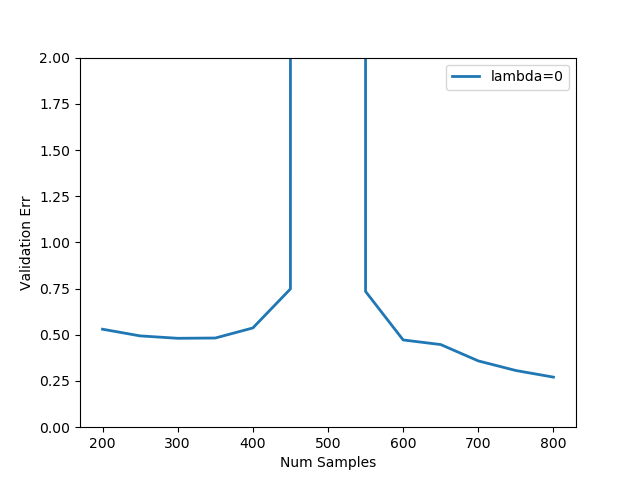
\includegraphics[width=0.65\linewidth]{04-doubledescent/unreg.png}
	\caption{Num of samples vs. validation error.}
	\centering
\end{figure}

The x-axis is the size of the training dataset (from 200 to 800); the y-axis is the MSE on the validation dataset. You should observe that the validation error increases and then decreases as we increase the sample size.

\textbf{Note:} When $n\approx d$, the test MSE could be very large. For better visualization, we let the if the test MSE goes out of scope in the plot for some points.